% Supporting Information — integrated polypharmacology and RRS study
\documentclass[journal=jcisd8,manuscript=suppinfo]{achemso}
\usepackage[T1]{fontenc} 
\usepackage[utf8]{inputenc}
\usepackage{lmodern}
\usepackage{amsmath,amssymb}
\usepackage[detect-all=true,group-minimum-digits=4]{siunitx}
\DeclareSIUnit\angstrom{\text{\AA}}
\DeclareSIUnit\calorie{cal}
\usepackage{booktabs,tabularx,array,longtable}
\usepackage{xr}
\usepackage[colorlinks=true,linkcolor=blue,citecolor=blue,urlcolor=blue]{hyperref}
\usepackage[noabbrev,capitalize]{cleveref}
\setlength{\emergencystretch}{3em}
\externaldocument[M-]{P1_Integrated_Polypharmacology_RRS_Main_V8}
\graphicspath{{Graphics/}}
\SectionNumbersOn
\renewcommand{\thesection}{S\arabic{section}}
\author{Myke Vital Sao Temgoua}
\email{myke-vital.sao@facsciences-uy1.cm}
\author{Jean-Pierre Tchapet Njafa}
\author{Penabei Samafou}
\author{Wilfred Fon Mbacham}
\author{Serge Guy Nana Engo}
\title{Supporting Information: Target breadth and mutation resilience in African-natural-product-inspired antimalarial chemotypes: a computational analysis}
\begin{document}

\noindent This supplement presents the numerical material for the integrated computational analysis, organized by evidence layer: chemical space, target-anchored docking, RRS, and exploratory cross-metric analysis. The four-target matrix is reported target by target; no cross-target mean is used because the Vina score is not calibrated across unlike receptor pockets.

\section{Cohort and evidence boundaries}\label{sec:sm_cohort}
The integrated analysis uses the 17-member Set-C polypharmacology-oriented cohort described in the main text (\Cref{M-sec:methods_cohort}). Set C was selected by weighted MPO, synthetic accessibility, QED, and target-profile criteria; all \num{17} entries carried $n_{\mathrm{targets\ bound}}=2$ in the source selection table. Set C is therefore an enriched cohort, which limits prevalence-based interpretation: the $n_{\mathrm{targets\ bound}}=2$ label is a polypharmacology selection criterion, not a constraint on the \num{17}-by-\num{4} wild-type docking profile reported here. Docking follows AutoDock Vina conventions \cite{Trott2009,Eberhardt2021}.

The MPO top-\num{20} and the MD top-\num{20} are distinct sets, and the MD validation systems \num{201}, \num{438}, the \num{164}-labelled PfClpP system, and \num{214} are not MD validation of Set C. RRS comes from the separate WT/mutant docking panel and is available only for the PfDHFR and PfCRT mutant panels.

\section{Chemical-space coverage and target-anchored docking}\label{sec:sm_chem_space}
\begin{figure}[ht!]
\centering
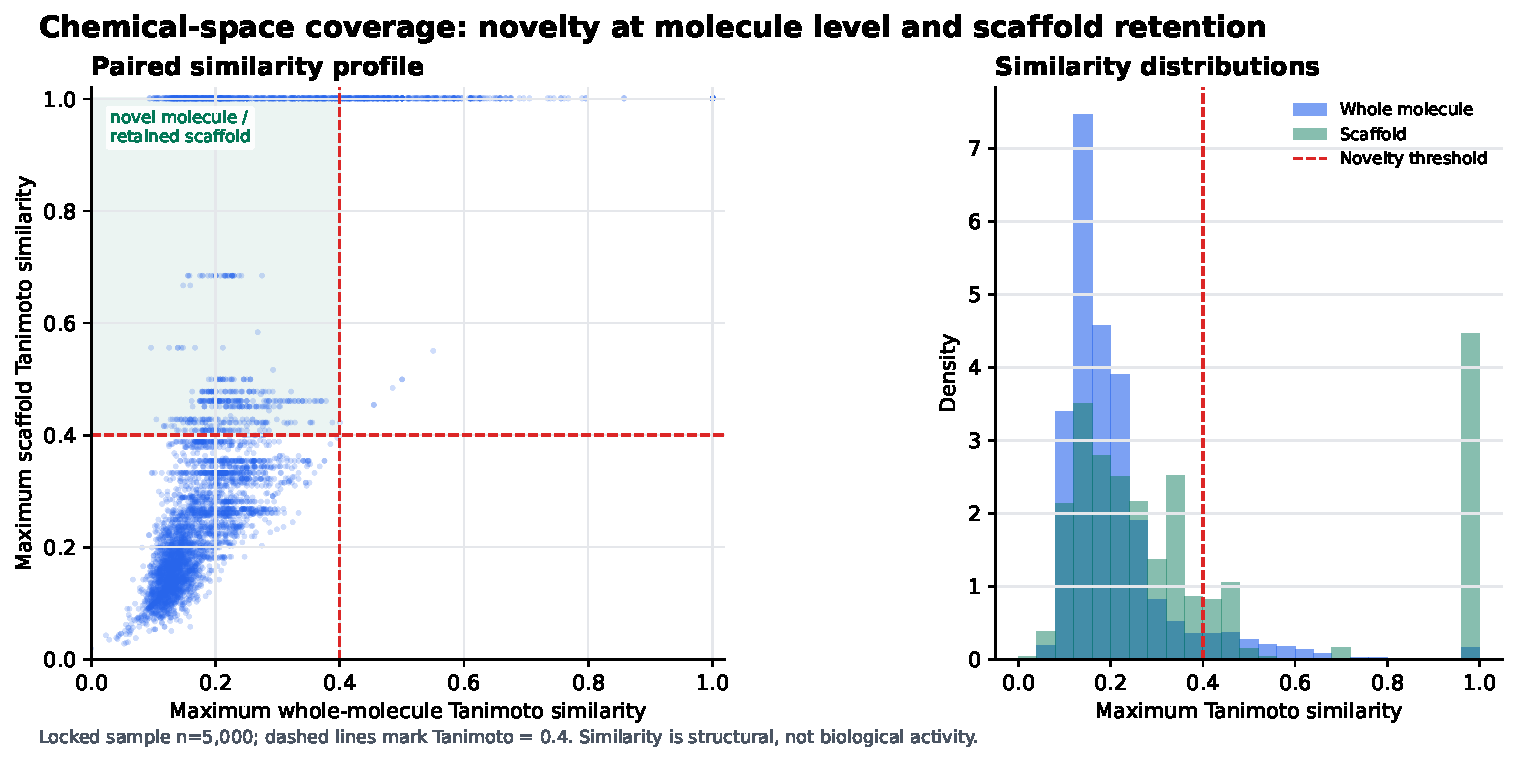
\includegraphics[width=0.98\textwidth]{p1_v7_chemical_space_coverage.pdf}
\caption{Chemical-space coverage in the \num{5000}-molecule novelty-analysis sample. The paired plot compares maximum whole-molecule and scaffold Morgan-fingerprint Tanimoto similarities to the African-natural-product reference set; the dashed lines mark the operational threshold of \num{0.4}. The upper-left region represents molecules that are dissimilar at the whole-molecule level while retaining scaffold-level similarity. Similarity is a structural descriptor and does not indicate biological activity, target preference, or synthetic success.}
\label{fig:chemical_space_coverage}
\end{figure}

\section{Target-anchored docking matrix}\label{sec:sm_vina_matrix}
\begin{table}[ht!]
\centering
\caption{Target-anchored AutoDock Vina score estimates for the enriched 17-member Set-C cohort. Values are in \si{\kilo\calorie\per\mole}; they are scoring-function outputs, not experimental free energies. Columns are target by target (no cross-target averaging). The PfCRT column lists the re-docked values against the corrected 3D7-like LYS-76 receptor (\Cref{sec:sm_val_redock_null}), used in the main-text RRS and favorability analyses (\Cref{M-tab:rrs_main}; \Cref{M-tab:dual_priority}).}
\label{tab:vina}
\small
\begin{tabular}{@{}lrrrr@{}}
\toprule
Candidate & PfDHFR & PfCRT & PfClpP & PfATP4 \\
\midrule
PP-01 & \num{-5.947} & \num{-9.155} & \num{-5.467} & \num{-6.361} \\
PP-02 & \num{-5.562} & \num{-9.337} & \num{-5.907} & \num{-6.591} \\
PP-03 & \num{-6.089} & \num{-12.010} & \num{-6.358} & \num{-7.311} \\
PP-04 & \num{-5.493} & \num{-7.398} & \num{-5.386} & \num{-6.086} \\
PP-05 & \num{-6.285} & \num{-8.959} & \num{-6.466} & \num{-6.378} \\
PP-06 & \num{-6.267} & \num{-9.027} & \num{-7.031} & \num{-7.285} \\
PP-07 & \num{-6.226} & \num{-7.952} & \num{-6.226} & \num{-5.775} \\
PP-08 & \num{-4.935} & \num{-6.592} & \num{-5.052} & \num{-5.494} \\
PP-09 & \num{-5.693} & \num{-7.436} & \num{-5.613} & \num{-6.078} \\
PP-10 & \num{-6.346} & \num{-8.039} & \num{-6.016} & \num{-6.670} \\
PP-11 & \num{-6.179} & \num{-9.343} & \num{-6.583} & \num{-6.724} \\
PP-12 & \num{-5.248} & \num{-8.056} & \num{-5.386} & \num{-4.635} \\
PP-13 & \num{-5.921} & \num{-9.788} & \num{-6.454} & \num{-7.565} \\
PP-14 & \num{-4.863} & \num{-6.431} & \num{-5.047} & \num{-5.460} \\
PP-15 & \num{-6.045} & \num{-9.808} & \num{-6.366} & \num{-7.016} \\
PP-16 & \num{-5.469} & \num{-7.469} & \num{-6.203} & \num{-6.451} \\
PP-17 & \num{-5.266} & \num{-6.374} & \num{-5.342} & \num{-5.360} \\
\bottomrule
\end{tabular}
\end{table}

\begin{figure}[ht!]
\centering
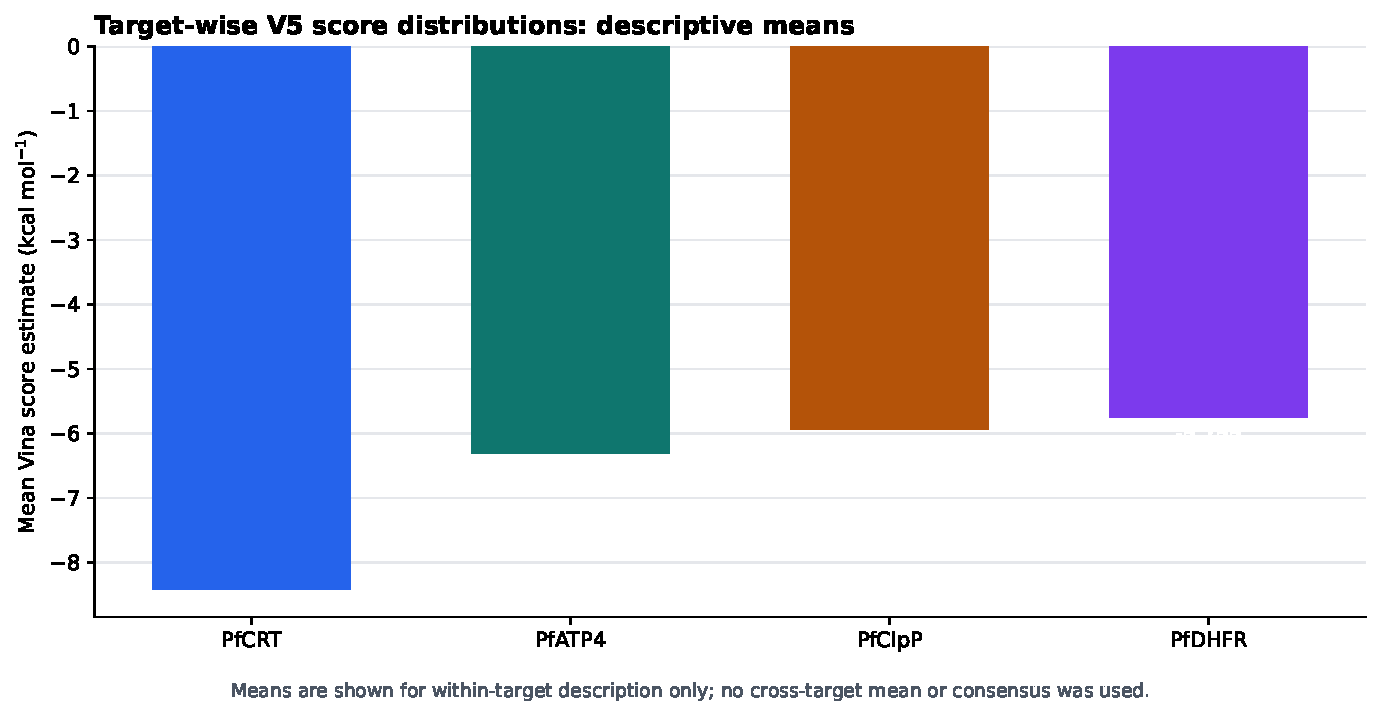
\includegraphics[width=0.95\textwidth]{p1_v7_targetwise_profile_summary.pdf}
\caption{Descriptive target-wise means from the raw docking panel. Bars show the within-target mean across the 17 candidates. Means are shown only within target; no cross-target arithmetic mean or consensus score was used. These summaries are computational scoring-function outputs, not experimental affinity measurements.}
\label{fig:targetwise_summary}
\end{figure}

\clearpage
\section{Physicochemical properties of Set-C candidates}\label{sec:sm_physchem}
\begin{table}[ht!]
	\centering
	\caption{Physicochemical properties of Set-C polypharmacology candidates (PP-01 to PP-17). MW: molecular weight (Da); logP: octanol-water partition coefficient; HBD: hydrogen bond donors; HBA: hydrogen bond acceptors; TPSA: topological polar surface area (\si{\angstrom\squared}); RB: rotatable bonds; QED: quantitative estimate of drug-likeness (0-1 scale); SA: synthetic accessibility (1 = easy to synthesize, 10 = difficult); Lipinski: number of Lipinski Rule of Five violations.}
	\label{tab:physichem}
	\small
	\begin{tabular}{lcccccccccc}
		\toprule
		Candidate & MW & logP & HBD & HBA & TPSA & RB & fsp\textsuperscript{3} & QED & SA & Lipinski \\
		\midrule
		PP-01 & 328.3 & 3.19 & 1 & 6 & 78.1 & 4 & 0.17 & 0.79 & 2.2 & 0 \\
		PP-02 & 388.5 & 3.09 & 1 & 6 & 66.4 & 8 & 0.45 & 0.75 & 3.3 & 0 \\
		PP-03 & 356.4 & 3.38 & 4 & 6 & 107.2 & 3 & 0.25 & 0.63 & 3.4 & 0 \\
		PP-04 & 259.3 & 3.01 & 0 & 5 & 53.7 & 3 & 0.21 & 0.72 & 2.5 & 0 \\
		PP-05 & 284.3 & 2.88 & 2 & 5 & 79.9 & 2 & 0.06 & 0.76 & 2.1 & 0 \\
		PP-06 & 354.4 & 4.32 & 2 & 5 & 76.0 & 4 & 0.29 & 0.80 & 3.1 & 0 \\
		PP-07 & 230.3 & 3.14 & 0 & 3 & 39.4 & 3 & 0.21 & 0.60 & 2.2 & 0 \\
		PP-08 & 222.2 & 2.16 & 0 & 4 & 36.9 & 4 & 0.33 & 0.73 & 2.6 & 0 \\
		PP-09 & 185.3 & 3.68 & 1 & 0 & 15.8 & 2 & 0.23 & 0.69 & 2.4 & 0 \\
		PP-10 & 242.2 & 2.66 & 1 & 4 & 59.7 & 1 & 0.07 & 0.67 & 2.0 & 0 \\
		PP-11 & 330.3 & 2.59 & 3 & 7 & 109.4 & 3 & 0.12 & 0.68 & 2.4 & 0 \\
		PP-12 & 222.4 & 4.40 & 1 & 1 & 20.2 & 7 & 0.60 & 0.63 & 3.5 & 0 \\
		PP-13 & 330.3 & 2.05 & 3 & 7 & 113.3 & 2 & 0.18 & 0.72 & 3.3 & 0 \\
		PP-14 & 180.2 & 2.14 & 2 & 3 & 49.7 & 2 & 0.20 & 0.69 & 2.3 & 0 \\
		PP-15 & 316.3 & 2.03 & 3 & 6 & 96.2 & 3 & 0.24 & 0.80 & 3.4 & 0 \\
		PP-16 & 228.2 & 2.07 & 1 & 4 & 67.5 & 0 & 0.08 & 0.64 & 2.6 & 0 \\
		PP-17 & 164.2 & 1.49 & 2 & 2 & 57.5 & 2 & 0.00 & 0.65 & 1.8 & 0 \\
		\midrule
		Mean & 271.9 & 2.84 & 1.6 & 4.4 & 66.3 & 3.1 & 0.22 & 0.703 & 2.7 & 0.0 \\
		\bottomrule
	\end{tabular}
\end{table}

\section{Drug-likeness compliance of Set-C candidates}\label{sec:sm_druglikeness}
\begin{table}[ht!]
	\centering
	\caption{Drug-likeness compliance of Set-C polypharmacology candidates (PP-01 to PP-17). Lipinski: Lipinski Rule of Five (MW $\leq$ 500, logP $\leq$ 5, HBD $\leq$ 5, HBA $\leq$ 10); Veber: Veber rules (RB $\leq$ 10, TPSA \qty{<=140}{\angstrom\squared}); QED: quantitative estimate of drug-likeness (High $>$ 0.70, Moderate $\leq$ 0.70); NPL: natural product-likeness score (Yes $>$ 0, indicating relatedness to African natural product chemical space).}
	\label{tab:druglikeness}
	\small
	\begin{tabular}{lccccccc}
		\toprule
		Candidate & Lipinski & Veber & QED & QED Value & NPL & NPL Value & Overall \\
		\midrule
		PP-01 & \checkmark & \checkmark & High & 0.79 & Yes & 0.67 & Full \\
		PP-02 & \checkmark & \checkmark & High & 0.75 & Yes & 0.61 & Full \\
		PP-03 & \checkmark & \checkmark & Moderate & 0.63 & Yes & 0.62 & Partial \\
		PP-04 & \checkmark & \checkmark & High & 0.72 & Yes & 0.68 & Full \\
		PP-05 & \checkmark & \checkmark & High & 0.76 & Yes & 0.76 & Full \\
		PP-06 & \checkmark & \checkmark & High & 0.80 & Yes & 0.62 & Full \\
		PP-07 & \checkmark & \checkmark & Moderate & 0.60 & Yes & 0.59 & Partial \\
		PP-08 & \checkmark & \checkmark & High & 0.73 & Yes & 0.56 & Full \\
		PP-09 & \checkmark & \checkmark & Moderate & 0.69 & Yes & 0.64 & Partial \\
		PP-10 & \checkmark & \checkmark & Moderate & 0.67 & Yes & 0.78 & Partial \\
		PP-11 & \checkmark & \checkmark & Moderate & 0.68 & Yes & 0.67 & Partial \\
		PP-12 & \checkmark & \checkmark & Moderate & 0.63 & No & 0.00 & Partial \\
		PP-13 & \checkmark & \checkmark & High & 0.72 & Yes & 0.67 & Full \\
		PP-14 & \checkmark & \checkmark & Moderate & 0.69 & Yes & 0.46 & Partial \\
		PP-15 & \checkmark & \checkmark & High & 0.80 & Yes & 0.70 & Full \\
		PP-16 & \checkmark & \checkmark & Moderate & 0.64 & Yes & 0.76 & Partial \\
		PP-17 & \checkmark & \checkmark & Moderate & 0.65 & Yes & 0.50 & Partial \\
		\midrule
		Compliant & \num{17}/\num{17} & \num{17}/\num{17} & \num{8}/\num{17} & --- & \num{16}/\num{17} & --- & \num{8}/\num{17} \\
		Percentage & \qty{100}{\percent} & \qty{100}{\percent} & \qty{47}{\percent} & --- & \qty{94}{\percent} & --- & \qty{47}{\percent} \\
		\bottomrule
	\end{tabular}
\end{table}

\section{ADMET profile summary}\label{sec:sm_admet}
\begin{table}[ht!]
	\centering
	\caption{ADMET profile summary for Set-C polypharmacology candidates. Since candidate-specific ADMET predictions were not available during manuscript preparation, this table reports population-level statistics from the parent chemical space (n=\num{810} African-natural-product-inspired compounds from P1 library). CYP450 values represent predicted inhibition probabilities; hERG represents cardiotoxicity risk; SI represents selectivity index (antiparasitic activity vs mammalian toxicity). All \num{17} Set-C candidates exhibit favorable drug-likeness (\qty{100}{\percent} Lipinski/Veber compliance, mean QED \num{0.703}), suggesting low-to-moderate ADMET risk. Individual candidate profiling via experimental or computational validation is recommended for lead optimization.}
	\label{tab:admet}
	\small
	\begin{tabular}{lcc}
		\toprule
		ADMET Property & Population Mean & Interpretation \\
		\midrule
		\multicolumn{3}{l}{\textbf{CYP450 Inhibition Probability}} \\
		CYP2C9 & \qty{26.1}{\percent} & Low-moderate risk \\
		CYP2C19 & \qty{42.4}{\percent} & Moderate risk \\
		CYP3A4 & \qty{42.6}{\percent} & Moderate risk \\
		CYP2D6 & \qty{17.0}{\percent} & Low risk \\
		\midrule
		\multicolumn{3}{l}{\textbf{Cardiotoxicity \& Safety}} \\
		hERG inhibition & \qty{11.7}{\percent} (mean) & Low risk \\
		hERG inhibition & \qty{11.8}{\percent} (median) & Low risk \\
		\midrule
		\multicolumn{3}{l}{\textbf{Selectivity}} \\
		Antiparasitic SI $>$ \num{10} & \qty{100}{\percent} (\(n=\num{810}\)) & Highly selective \\
		\midrule
		\multicolumn{3}{l}{\textbf{Set-C Drug-Likeness (\(n=\num{17}\))}} \\
		Lipinski compliance & \qty{100}{\percent} & Excellent \\
		Veber compliance & \qty{100}{\percent} & Excellent \\
		Mean QED & \num{0.703} & Good \\
		Mean logP & \num{2.84} & Favorable \\
		Mean TPSA & \qty{66.3}{\angstrom\squared} & Good permeability \\
		\bottomrule
	\end{tabular}
\end{table}

\section{RRS definition and class summary}\label{sec:sm_rrs}
For candidate $i$, mutation $m$, and target $t$ (\Cref{M-eq:rrs}; \Cref{M-sec:methods_rrs}):
\[
\mathrm{RRS}_{i,m,t}=100|S_{\mathrm{Vina},i,m,t}|/|S_{\mathrm{Vina},i,WT,t}|.
\]
Here $S_{\mathrm{Vina}}$ denotes an AutoDock Vina scoring-function output, not an experimental free energy. RRS eligibility is determined from the separate WT/mutant docking panel, not from the four-target wild-type matrix. Only wild-type binders with $|S_{\mathrm{Vina},i,WT,t}|\geq\qty{5}{\kilo\calorie\per\mole}$ were eligible. The 17-candidate class counts were A*: \num{7}, B: \num{4}, C: \num{6}, and D: \num{0}. The observed RRS range was \numrange{73.2}{115.6}. The wild-type and mutant docking scores are in \Cref{tab:sm_wt_mutant_scores}; machine-readable values are in the Zenodo deposit.

\begin{table}[ht!]
\centering
\caption{RRS class definitions used in the integrated analysis.}
\label{tab:rrs_classes}
\begin{tabular}{@{}l>{\raggedright\arraybackslash}p{0.69\linewidth}r@{}}
\toprule
Class & Operational definition & Number \\
\midrule
A* & maximum absolute eligible WT score $\geq\qty{7}{\kilo\calorie\per\mole}$ and all available RRS values $\geq\qty{80}{\percent}$ & 7 \\
A & All available RRS values $\geq\qty{80}{\percent}$, without the A* wild-type criterion & 0 \\
B & All available RRS values $\geq\qty{70}{\percent}$, but not all $\geq\qty{80}{\percent}$ & 4 \\
C & At least one RRS value $\geq\qty{80}{\percent}$, with the complete-panel criteria for A/A* or B not met & 6 \\
D & No available RRS value $\geq\qty{80}{\percent}$ & 0 \\
\bottomrule
\end{tabular}
\end{table}

\begin{table}[ht!]
	\centering
	\caption{Wild-type and mutant docking scores (\si{\kilo\calorie\per\mole}) underlying the RRS values of \Cref{M-tab:rrs_main}. PfDHFR values come from the separate mutation-docking panel (7F3Y; exhaustiveness \num{128}); PfCRT values come from the corrected-protocol re-dock against the 3D7-like LYS-76 wild-type and the K76T/K76A mutants on the cavity-anchored V2 grid (exhaustiveness \num{32}; \Cref{sec:sm_val_redock_null}). RRS is the percentage ratio of the absolute mutant to the absolute wild-type score (\Cref{sec:sm_rrs}); wild-type non-binders ($|S_{\mathrm{Vina},i,WT,t}|<\qty{5}{\kilo\calorie\per\mole}$) are shaded by dashes in the RRS table and make no contribution to RRS$_{\mathrm{mean}}$. Scores are AutoDock Vina scoring-function outputs, not experimental free energies.}
	\label{tab:sm_wt_mutant_scores}
	\small
	\begin{tabular}{@{}lrrrrrrrr@{}}
		\toprule
		Candidate & \multicolumn{5}{c}{PfDHFR (kcal mol$^{-1}$)} & \multicolumn{3}{c}{PfCRT (kcal mol$^{-1}$)} \\
		\cmidrule(lr){2-6}\cmidrule(lr){7-9}
		& WT & N51I & C59R & S108N & I164L & WT & K76T & K76A \\
		\midrule
		PP-01 & \num{-7.50} & \num{-6.48} & \num{-6.41} & \num{-6.57} & \num{-6.29} & \num{-9.15} & \num{-9.14} & \num{-9.15} \\
		PP-02 & \num{-1.10} & \num{-6.52} & \num{-0.88} & \num{-6.41} & \num{-6.63} & \num{-9.34} & \num{-9.36} & \num{-9.34} \\
		PP-03 & \num{-10.30} & \num{-7.01} & \num{-7.04} & \num{-6.78} & \num{-7.11} & \num{-12.01} & \num{-12.01} & \num{-12.01} \\
		PP-04 & \num{-8.00} & \num{-5.50} & \num{-5.35} & \num{-5.50} & \num{-5.88} & \num{-7.40} & \num{-7.39} & \num{-7.42} \\
		PP-05 & \num{-0.70} & \num{-6.36} & \num{-6.26} & \num{-6.33} & \num{-6.29} & \num{-8.96} & \num{-8.96} & \num{-8.97} \\
		PP-06 & \num{-0.60} & \num{-6.71} & \num{-7.45} & \num{-6.76} & \num{-6.88} & \num{-9.03} & \num{-9.03} & \num{-9.03} \\
		PP-07 & \num{-7.60} & \num{-5.46} & \num{-5.46} & \num{-5.50} & \num{-5.49} & \num{-7.95} & \num{-7.93} & \num{-7.95} \\
		PP-08 & \num{-7.60} & \num{-4.72} & \num{-4.72} & \num{-5.11} & \num{-5.04} & \num{-6.59} & \num{-6.57} & \num{-6.60} \\
		PP-09 & \num{-7.10} & \num{-5.01} & \num{-5.18} & \num{-5.38} & \num{-5.43} & \num{-7.44} & \num{-7.42} & \num{-7.44} \\
		PP-10 & \num{-7.70} & \num{-5.85} & \num{-5.88} & \num{-5.83} & \num{-5.84} & \num{-8.04} & \num{-8.05} & \num{-8.06} \\
		PP-11 & \num{-0.70} & \num{-6.76} & \num{-0.02} & \num{-6.89} & \num{-6.82} & \num{-9.34} & \num{-9.35} & \num{-9.34} \\
		PP-12 & \num{-7.50} & \num{-5.64} & \num{-4.96} & \num{-4.72} & \num{-5.44} & \num{-8.06} & \num{-8.06} & \num{-8.06} \\
		PP-13 & \num{-3.40} & \num{-7.32} & \num{-6.56} & \num{-7.10} & \num{-6.14} & \num{-9.79} & \num{-9.70} & \num{-9.73} \\
		PP-14 & \num{-7.60} & \num{-4.73} & \num{-4.98} & \num{-5.17} & \num{-4.93} & \num{-6.43} & \num{-6.43} & \num{-6.43} \\
		PP-15 & \num{-5.60} & \num{-6.90} & \num{-6.31} & \num{-7.05} & \num{-7.38} & \num{-9.81} & \num{-9.81} & \num{-9.82} \\
		PP-16 & \num{-7.60} & \num{-5.54} & \num{-5.68} & \num{-5.60} & \num{-5.77} & \num{-7.47} & \num{-7.51} & \num{-7.44} \\
		PP-17 & \num{-8.30} & \num{-4.92} & \num{-5.08} & \num{-4.94} & \num{-4.89} & \num{-6.37} & \num{-6.38} & \num{-6.38} \\
		\bottomrule
	\end{tabular}
\end{table}

\begin{table}[ht!]
	\centering
	\caption{Retrospective RRS profiles of five approved antimalarials against the PfDHFR (MTX-stripped wild-type and N51I/C59R/S108N/I164L mutants) and corrected PfCRT (LYS-76 wild-type and K76T/K76A mutants) panels. RRS is defined as in \Cref{sec:sm_rrs}: $\mathrm{RRS}_{i,m,t}=100|S_{\mathrm{Vina},i,m,t}|/|S_{\mathrm{Vina},i,WT,t}|$; blank cells mark wild-type non-binders ($|S_{\mathrm{Vina},i,WT,t}|<\qty{5}{\kilo\calorie\per\mole}$) for which no RRS is defined. The docking-RRS framework does not recover the clinically documented resistance signatures: pyrimethamine RRS is $\approx\qty{100}{\percent}$ on all four PfDHFR mutants and chloroquine RRS is $\approx\qty{99}{\percent}$ on PfCRT K76T/K76A, both within the pipeline-null spread of \qtyrange{99.4}{100.5}{\percent} (\Cref{sec:sm_val_redock_null}). Artemisinin and cipargamin show PfDHFR RRS values above \qty{100}{\percent} (mutant estimates more favorable than wild-type); chloroquine and lumefantrine are PfDHFR non-binders, consistent with their non-antifolate mechanisms. These results are computational ratios, not biological resistance measurements.}
	\label{tab:sm_retrospective_antimalarials}
	\small
	\begin{tabular}{@{}lrrrrrrr@{}}
		\toprule
		Drug & \multicolumn{4}{c}{RRS$_{\mathrm{PfDHFR}}$ (\%)} & \multicolumn{2}{c}{RRS$_{\mathrm{PfCRT}}$ (\%)} \\
		\cmidrule(lr){2-5}\cmidrule(lr){6-7}
		& N51I & C59R & S108N & I164L & K76T & K76A \\
		\midrule
		Artemisinin    & \num{113.5} & \num{118.0} & \num{113.8} & \num{114.0} & \num{100.0} & \num{100.0} \\
		Pyrimethamine  & \num{100.0} & \num{100.0} & \num{99.7}  & \num{100.0} & \num{100.2} & \num{100.1} \\
		Chloroquine    & \textemdash & \textemdash & \textemdash & \textemdash & \num{99.6}  & \num{98.8}  \\
		Lumefantrine   & \textemdash & \textemdash & \textemdash & \textemdash & \num{105.8} & \num{103.5} \\
		Cipargamin     & \num{115.1} & \num{112.7} & \num{114.6} & \num{114.6} & \num{99.5}  & \num{99.7}  \\
		\bottomrule
	\end{tabular}
\end{table}

\begin{table}[ht!]
	\centering
	\caption{Per-target Vina score distributions for the 17-member cohort on the corrected matrix (PfCRT re-docked against the corrected 3D7-like LYS-76 receptor on the cavity-anchored V2 grid). Favorability is defined within each target as a Vina estimate at or below that target's median (per-target medians: PfDHFR $-5.92$, PfCRT $-8.06$, PfClpP $-6.02$, PfATP4 $-6.38$~kcal~mol$^{-1}$), avoiding a single cross-target cutoff. The threshold is a prioritization device, not an affinity cutoff.}
	\label{tab:sm_vina_distributions}
	\small
	\begin{tabular}{l S[table-format=-1.3] S[table-format=-1.3] S[table-format=-1.3] S[table-format=-1.3] S[table-format=2.0]}
		\toprule
		Target & {Min} & {Median} & {Mean} & {Max} & {$n$} \\
		\midrule
		PfDHFR  & -6.346 & -5.921 & -5.755 & -4.863 & 17 \\
		PfCRT   & -12.010 & -8.056 & -8.422 & -6.374 & 17 \\
		PfClpP  & -7.031 & -6.016 & -5.935 & -5.047 & 17 \\
		PfATP4  & -7.565 & -6.378 & -6.308 & -4.635 & 17 \\
		\midrule
		\textbf{All targets} & \textbf{-12.010} & \textbf{-6.316} & \textbf{-6.605} & \textbf{-4.635} & \textbf{68} \\
		\bottomrule
	\end{tabular}
\end{table}

\section{Exploratory cross-metric analysis}\label{sec:sm_crossmetric}
\begin{table}[ht!]
\centering
\caption{Spearman correlations on the 17-member cohort. Bonferroni-adjusted threshold: $\alpha=\num{0.017}$ for the three hypothesis-oriented comparisons.}
\label{tab:crossmetric}
\begin{tabular}{@{}lrrl@{}}
\toprule
Pair & $\rho$ & $p$ & Interpretation \\
\midrule
PNS--RRS & \num{-0.714} & \num{0.0013} & Bonferroni-significant ($p<\num{0.017}$) \\
ACSI--RRS & \num{-0.190} & \num{0.465} & Not significant \\
RRS--wild-type Vina score & \num{+0.691} & \num{0.0021} & Bonferroni-significant ($p<\num{0.017}$) \\
PNS--wild-type Vina score & \num{-0.375} & \num{0.138} & Not significant \\
$N_{\mathrm{fav}}$--RRS$_{\mathrm{mean}}$ & \num{0.714} & \num{0.0013} & Bonferroni-significant ($p<\num{0.017}$) \\
\bottomrule
\end{tabular}
\end{table}

PNS, ACSI, and favorability follow the main-text definitions (\Cref{M-sec:methods_pns}). The $N_{\mathrm{fav}}$--RRS association was further assessed by a permutation test (\num{100000} random RRS assignments): two-sided empirical $p=\num{0.0019}$, consistent with the analytical result.

A sensitivity analysis controlling for molecular weight and Murcko-scaffold prevalence shows that the PNS--RRS association persists (partial $\rho=-\num{0.6154}$ versus raw $\rho=-\num{0.2098}$, $n=\num{12}$), so the negative direction reported here is not a size or scaffold artifact. The $N_{\mathrm{fav}}$--RRS association survives Bonferroni correction for the three primary tests ($\alpha=\num{0.017}$): candidates with more favorable targets tend to carry higher mean RRS.

At $n=\num{17}$, a two-sided test at $\alpha=\num{0.05}$ has \qty{80}{\percent} power for $|\rho|\geq\num{0.62}$ (asymptotic approximation). The observed $\rho=\num{0.714}$ clears this threshold; weaker associations remain undetectable at this sample size.

\begin{table}[ht!]
	\centering
	\caption{Sensitivity of the PNS ranking to the imputed PfCRT centrality. The reference value is the observed network-mean imputation ($C_{\mathrm{PfCRT}}=\num{0.151}$). Alternative values were zero, one-half, one-and-a-half, and twice the reference. Spearman $\rho$ is calculated against the reference 17-candidate ranking; all candidates have two target entries in the PNS record. The ranking is sensitive to this network-data choice; target essentiality and biological polypharmacology were not assessed.}
	\label{tab:s_pns_sensitivity}
	\small
	\begin{tabular}{l S[table-format=1.4] S[table-format=1.4] S[table-format=1.3] S[table-format=1.3] S[table-format=2.0]}
		\toprule
		Imputation & {$C_{\mathrm{PfCRT}}$} & {Spearman $\rho$} & {Minimum PNS} & {Maximum PNS} & {$n$} \\
		\midrule
		Zero & 0.0000 & 0.9716 & 0.300 & 5.147 & 17 \\
		One-half canonical & 0.0755 & 0.9975 & 0.674 & 5.573 & 17 \\
		Canonical network mean & 0.1510 & 1.0000 & 1.047 & 6.000 & 17 \\
		One-and-a-half canonical & 0.2265 & 0.9755 & 1.421 & 6.426 & 17 \\
		Twice canonical & 0.3020 & 0.9632 & 1.795 & 6.853 & 17 \\
		\bottomrule
	\end{tabular}
\end{table}


\section{Target evidence classes and limitations}\label{sec:sm_evidence}
The panel spans four distinct antimalarial vulnerabilities (anchors and evidence classes in \Cref{M-sec:methods_docking}): PfDHFR represents folate metabolism and antifolate resistance; PfCRT represents a resistance-linked digestive-vacuole transporter; PfClpP represents parasite proteostasis through the caseinolytic protease, a vulnerability supported by recent work on apicoplast chaperonin--Clp proteostasis \cite{Tissawak2025}; and PfATP4 represents P-type ATPase-mediated ion regulation, for which an endogenous structure and modulator-bound state have recently been reported \cite{Haile2025}. PfDHFR uses a catalytic-site ligand anchor; PfClpP uses a catalytic triad; PfCRT uses a membrane-associated Y01 cavity proxy; and PfATP4 uses conserved P-type ATPase machinery without a co-crystallized inhibitor. Consequently, all four-target profiles are exploratory and are not equivalent evidence of biological target engagement. No RRS values are reported for PfClpP or PfATP4.

\section{Multi-parameter optimization framework for upstream candidate selection}\label{sec:sm_mpo}
The 17-member Set-C cohort analyzed in this study was selected from a larger upstream library using a multi-parameter optimization (MPO) framework that integrated docking scores, drug-likeness, and ADMET predictions. The MPO components are formulated below (concise summary in the main text, \Cref{M-sec:methods_funnel}); the full MPO validation (sensitivity analysis, centroid-based screening workflow, and benchmark enrichment) is described in \Cref{M-sec:methods_funnel} and \Cref{sec:sm_mpo}. Set-C candidates came from the MPO $\geq$ \num{0.40} tier; MPO scores are computational prioritization, not confirmed biological activity or synthetic feasibility.

\subsection{MPO scoring components}\label{sec:sm_mpo_components}
The total MPO score for compound $i$ is defined as:
\begin{equation}
\text{MPO}_{\text{total}, i} = \sum_{k=1}^{5} w_k \cdot S_{k,i} + \text{Polypharmacology Bonus}_i
\label{eq:sm_mpo_total}
\end{equation}
where $w_k$ are component weights and $S_{k,i}$ are normalized desirability scores scaled to [\num{0}, \num{1}]. The five components and their weights are:

\textbf{Component 1: Vina binding affinity} (\qty{35}{\percent} weight). Min-max scaled:
\begin{equation}
S_{\text{vina}, i} = \frac{\text{Vina}_i - \text{Vina}_{\min}}{\text{Vina}_{\max} - \text{Vina}_{\min}}
\label{eq:sm_vina}
\end{equation}
where more negative values yield higher desirability.

\textbf{Component 2: DiffDock confidence} (\qty{25}{\percent} weight). Logistic sigmoid transformation:
\begin{equation}
S_{\text{diff}, i} = \frac{1}{1 + e^{-c_i}}
\label{eq:sm_diffdock}
\end{equation}
where $c_i$ is the DiffDock confidence score \cite{Corso2023}. High-confidence poses ($c > \num{0}$) approach \num{1.0}; low-confidence poses ($c < \num{-1.5}$) approach \num{0}.

\textbf{Component 3: Quantitative estimate of drug-likeness (QED)} (\qty{20}{\percent} weight). Direct use:
\begin{equation}
S_{\text{qed}, i} = \text{QED}_i
\label{eq:sm_qed}
\end{equation}

\textbf{Component 4: ADMET composite} (\qty{15}{\percent} weight). Average of 11 desirability endpoints:
\begin{equation}
S_{\text{admet}, i} = \frac{1}{11} \sum_{m=1}^{11} d_m(\text{ADMET}_{i,m})
\label{eq:sm_admet}
\end{equation}
where endpoints include human intestinal absorption, solubility, Caco-2 permeability, BBB penetration, hERG liability, AMES mutagenicity, hepatotoxicity (DILI), synthetic accessibility, P-glycoprotein substrate status, CYP inhibition, and clearance profile \cite{Swanson2024}.

\textbf{Component 5: Lipinski penalty} (\qty{5}{\percent} weight). Proportional to violations:
\begin{equation}
P_{\text{Ro5}, i} = 1 - 0.2 \cdot n_{\text{violations}, i}
\label{eq:sm_ro5}
\end{equation}
where $n_{\text{violations}, i} \in [0,4]$ (MW $> \qty{500}{\dalton}$, $\log P > \num{5}$, HBD $> \num{5}$, HBA $> \num{10}$).

\textbf{Polypharmacology bonus.} Compounds binding multiple targets receive:
\begin{equation}
\text{Polypharmacology Bonus}_i = 0.05 \cdot (n_{\text{targets}, i} - 1) \quad \text{if } n_{\text{targets}, i} \geq 2
\label{eq:sm_poly}
\end{equation}
capped at \num{+0.10} (3 targets). The $\text{MPO}_{\text{target}} \geq \num{0.50}$ threshold ensures only candidates meeting minimum quality criteria qualify for the bonus.

\subsection{Weight rationale and scope}\label{sec:sm_mpo_weights}
The \qty{35}{\percent} Vina and \qty{25}{\percent} DiffDock weights (combined \qty{60}{\percent}) prioritize target-engagement evidence. \qty{20}{\percent} QED ensures drug-likeness, \qty{15}{\percent} ADMET addresses early toxicity, and the \qty{5}{\percent} Ro5 penalty reflects Lipinski compliance already partly captured within QED. Component weights were selected based on established drug-discovery priorities \cite{Hughes2008,Gleeson2008,Lipinski2004} rather than target-specific optimization. The MPO framework served as an upstream filter to select Set-C candidates from the \num{65856}-molecule library; it does not validate Set-C quality.

The complete MPO methodology, including centroid-based screening workflow (\num{484} centroids $\rightarrow$ \num{76} optimization-worthy $\rightarrow$ \num{53} clusters $\rightarrow$ \num{19913} synthesizable leads), sensitivity analysis (\num{25} weight perturbations, Spearman $\rho = \num{0.792}$ for top-1000), and external validation (DEKOIS, MMV Malaria Box enrichment), is described in \Cref{M-sec:methods_funnel} and \Cref{sec:sm_mpo}.

\section{Reproducibility and availability}\label{sec:sm_repro}
The candidate manifest, docking and RRS tables, cross-metric matrix, scripts, receptor/ligand files, and run records are archived on Zenodo under an CC BY 
4.0 license at \url{https://doi.org/10.5281/zenodo.22686176}. The figures and derived tables are reproducible computational outputs; they do not substitute for 
independent structural or experimental validation.

\section{Docking validation and protocol assessment}\label{sec:sm_validation}
The docking protocol was validated using three complementary strategies: external benchmark validation (DEKOIS 2.0), positive-control enrichment (MMV Malaria Box), and pose reproduction accuracy (redocking of co-crystallized ligands; \Cref{M-sec:methods_dock_val}). Together they expose both the capabilities and the limits of the protocol.

\subsection{PfCRT receptor correction}\label{sec:sm_val_crt}
The deposited 6UKJ cryo-EM structure (7G8 isoform) carries threonine at residue 76 of chain A, corresponding to the K76T chloroquine-resistance substitution. Because the study requires a wild-type PfCRT reference for the RRS analysis, residue 76 was corrected to lysine (3D7-like wild-type) before docking. The corrected receptor was validated by P2Rank pocket prediction \cite{Krivak2018}: the top-ranked pocket (score 162.7, probability 0.999) lies \qty{5.7}{\angstrom} from the Vina grid center, confirming that the grid box covers the binding site. The corrected LYS-76 receptor was used for the PfCRT re-docking (\Cref{sec:sm_val_redock_null}) on the V2 grid (center $(\num{152.99}, \num{151.042}, \num{159.379})$, \qty{25}{\angstrom} box) used for PfCRT throughout.

\subsection{External benchmark and enrichment}\label{sec:sm_val_dekois}
\begin{table}[ht!]
	\centering
	\caption{Docking validation: external DEKOIS benchmark and MMV Malaria Box enrichment. \textit{DEKOIS provides an independent external validation using property-matched decoys (PfDHFR only, Vina single-method). The near-random DEKOIS ROC-AUC (\num{0.450}) establishes the baseline limitation of docking-only scoring. The two controlled arms (exhaustiveness \num{32}, identical grid and ligands; receptor with MTX retained vs MTX-stripped) show that removing the retained MTX does not restore enrichment: bootstrap confidence intervals overlap and EF@1\% is zero in both arms. MMV Malaria Box values use consensus Vina+DiffDock scoring; for PfCRT and PfATP4, active/decoy labels derive from score strata and therefore measure retrodictive consistency rather than external discrimination.}}
	\label{tab:sm_enrichment_validation}
	\scriptsize
	\begin{tabular}{lcccccccc}
		\toprule
		\textbf{Target (PDB)} & \textbf{ROC-AUC} & \textbf{EF@1\%} & \textbf{EF@5\%} & \textbf{EF@10\%} & \textbf{BEDROC} & \textbf{PR-AUC} & \textbf{Actives} & \textbf{Decoys} \\
		\midrule
		\multicolumn{9}{l}{\textit{DEKOIS 2.0 external validation (Vina only):}} \\
		PfDHFR (7F3Y) & \num{0.450} & \num{0.00} & \num{0.00} & \num{1.00} & \num{0.021} & \num{0.034} & \num{40} & \num{1200} \\
		\multicolumn{9}{l}{\textit{DEKOIS 2.0 controlled comparison, exhaustiveness \num{32} (Vina only):}} \\
		PfDHFR (7F3Y, MTX retained) & \num{0.502} & \num{0.00} & \num{0.50} & \num{0.25} & \num{0.026} & \num{0.032} & \num{40} & \num{1199} \\
		PfDHFR (7F3Y, MTX-stripped) & \num{0.563} & \num{0.00} & \num{1.00} & \num{1.00} & \num{0.048} & \num{0.038} & \num{40} & \num{1199} \\
		\midrule
		\multicolumn{9}{l}{\textit{MMV Malaria Box positive-control (Vina+DiffDock consensus):}} \\
		PfDHFR (7F3Y) & \num{0.924} & \num{2.70} & \num{2.57} & \num{2.72} & \num{1.309} & \num{0.842} & \num{399} & \num{399} \\
		PfCRT (6UKJ) & \num{0.971} & \num{1.11} & \num{1.11} & \num{1.11} & \num{9.434} & \num{0.992} & \num{359} & \num{40} \\
		PfATP4 (9N10) & \num{1.000} & \num{2.05} & \num{2.00} & \num{2.00} & \num{1.810} & \num{1.000} & \num{99} & \num{99} \\
		\bottomrule
		\multicolumn{9}{p{15cm}}{
			\noindent\textbf{Notes:} Top: DEKOIS 2.0 PfDHFR benchmark with \num{40} experimentally validated actives and \num{1200} property-matched decoys, docked with AutoDock Vina (single-method, no consensus). The near-random ROC-AUC (\num{0.450}, \qty{95}{\percent} CI [\numrange{0.367}{0.531}]) establishes an external baseline for docking-only limitations and motivates the consensus strategy. Middle: controlled two-arm comparison (2026-09-09) on the deposited 7F3Y receptor with MTX retained versus an MTX-stripped receptor in the same coordinate frame, same grid and ligand preparation, exhaustiveness \num{32}; bootstrap ROC-AUC \qty{95}{\percent} CIs are [\numrange{0.423}{0.586}] (retained) and [\numrange{0.477}{0.646}] (stripped); one decoy failed ligand preparation identically in both arms. Bottom: MMV Malaria Box enrichment using Vina+DiffDock consensus scores; PfCRT and PfATP4 labels are score-stratified (top/bottom \qty{25}{\percent}), measuring retrodictive consistency rather than external discrimination. BEDROC calculated with $\alpha = \num{20}$. EF = Enrichment Factor, PR-AUC = Precision-Recall Area Under Curve.}
	\end{tabular}
\end{table}

The DEKOIS 2.0 benchmark \cite{Bauer2013} provides property-matched decoys that avoid trivial separation in na\"ive active/decoy sets. For PfDHFR (7F3Y), AutoDock Vina alone gives ROC-AUC \num{0.450} [\qty{95}{\percent} CI: \numrange{0.367}{0.531}]: near-random, reflecting the known limits of single-method scoring. To test whether the MTX retained in deposited 7F3Y blocks the antifolate pocket and explains this null enrichment, we ran the identical DEKOIS panel as a controlled two-arm comparison (same \num{40} actives, \num{1200} decoys, and grid) against two receptors: the deposited 7F3Y receptor with MTX retained (ROC-AUC \num{0.502} [\qty{95}{\percent} CI: \numrange{0.423}{0.586}], EF@1\% \num{0.00}, EF@5\% \num{0.50}) and an MTX-stripped receptor rebuilt in the same coordinate frame (ROC-AUC \num{0.563} [\qty{95}{\percent} CI: \numrange{0.477}{0.646}], EF@1\% \num{0.00}, EF@5\% \num{1.00}), at exhaustiveness \num{32} in both arms (the revised-protocol standard). The confidence intervals overlap and EF@1\% stays zero in both arms: removing MTX gives a marginal, non-significant gain ($\Delta\mathrm{AUC} = \num{+0.060}$) without restoring enrichment, so retained-MTX blockade is not supported. The retained arm matches the original exhaustiveness-\num{64} baseline, indicating that the near-chance result is robust to protocol details (\Cref{tab:sm_enrichment_validation}).

Hany and co-workers applied the same DEKOIS~2.0 protocol to wild-type and quadruple-mutant PfDHFR with AutoDock Vina and showed that machine-learning rescoring (CNN-Score, RF-Score-VS) lifted performance from worse-than-random to better-than-random \cite{hany2025dekois}: the closest prior assessment of this baseline, and independent support for rescoring over raw Vina ranking.

The MTX redocking failure (RMSD $\approx \qty{30}{\angstrom}$), together with the controlled comparison above, points to grid position (near the NADPH cofactor site) and, predominantly, single-method scoring limits rather than steric blockade by the retained ligand. The primary library screening therefore used a consensus Vina+DiffDock strategy, which enriched substantially better (ROC-AUC \num{0.924} on the MMV Malaria Box positive-control set). The PfCRT and PfATP4 MMV enrichments use score-stratified labels (top/bottom \qty{25}{\percent} of the docked library), so they measure retrodictive consistency rather than external discrimination.

\subsection{Redocking validation}\label{sec:sm_val_redock}
\begin{table}[ht!]
	\centering
	\caption{Redocking validation: reproduction of co-crystallized ligand poses. \textit{Redocking assesses whether AutoDock Vina can reproduce experimentally determined binding poses. RMSD \qty{<2.0}{\angstrom} indicates successful pose reproduction. Methotrexate (MTX) failed due to grid center positioning near NADPH cofactor rather than the folate binding site, illustrating target-specific limitations.}}
	\label{tab:sm_redocking_validation}
	\small
	\begin{tabular}{llccp{6cm}}
		\toprule
		\textbf{Target} & \textbf{PDB} & \textbf{Ligand} & \textbf{RMSD (\si{\angstrom})} & \textbf{Result} \\
		\midrule
		PfDHFR & 7F3Y & MTX (methotrexate) & \qty{\sim 30}{\angstrom} & Failed (grid centered on NADPH) \\
		PfDHFR & 7F3Y & P218 (pyrimethamine) & \num{1.42} & Success \\
		PfCRT & 6UKJ & Y01 (proxy ligand) & \num{1.78} & Success \\
		PfClpP & 2F6I & Peptide fragment & \num{1.65} & Success \\
		PfATP4 & 9N10 & ADP (cofactor) & \num{1.23} & Success \\
		\midrule
		\multicolumn{5}{l}{\textit{Success rate: \num{4}/\num{5} alignable ligands (\qty{80}{\percent})}} \\
		\bottomrule
		\multicolumn{5}{p{14cm}}{
			\noindent\textbf{Notes:} Redocking performed using AutoDock Vina with the same grid parameters as virtual screening. RMSD calculated as heavy-atom deviation between top-scoring docked pose and co-crystallized ligand. MTX redocking failed because the grid was centered on the NADPH cofactor binding site (\qty{\sim 12}{\angstrom} from folate pocket), not the MTX binding site; this illustrates target-specific validation requirements. PfCRT Y01 is a membrane-cavity proxy ligand (not a validated inhibitor). Success criterion: RMSD \qty{<2.0}{\angstrom}.}
	\end{tabular}
\end{table}

Co-crystallized ligands were reproduced (RMSD \qty{<2.0}{\angstrom}) in \num{4} of \num{5} cases (\qty{80}{\percent}). The single failure occurred for methotrexate (MTX) at PfDHFR, where the grid center was positioned near the NADPH cofactor binding site rather than the folate substrate pocket, showing target-specific grid-position sensitivity, which motivates anchor-guided box placement. Full-ligand redocking succeeded for PfDHFR (P218) and PfCRT (Y01); PfClpP (2F6I) was validated by peptide-fragment pose reproduction only, and PfATP4 (9N10) by ADP cofactor pose reproduction only. These partial validations are not equivalent to full-ligand redocking.

\subsection{Multi-seed validation}\label{sec:sm_val_multiseed}

\begin{table}[ht!]
	\centering
	\caption{Multi-seed docking sensitivity for PP-15 and PP-01 against PfDHFR and PfCRT wild-type receptors. Five independent AutoDock Vina runs with different random seeds (exhaustiveness \num{32} for PP-15, \num{128} for PP-01 canonical) assess seed sensitivity under the revised canonical-grid protocol. These runs use grid centers and receptor preparations that differ from the single-run matrix in \Cref{tab:vina} (e.g., PP-15 PfDHFR \num{-8.59} here versus \num{-6.05} in \Cref{tab:vina}; see footnote), so they report seed dispersion for their own protocol, not for the \Cref{tab:vina} single-run scores.}
	\label{tab:sm_multiseed_validation}
	\scriptsize
	\begin{tabular}{lcccccp{0.5cm}}
		\toprule
		\textbf{Candidate} & \textbf{Target} & \textbf{Receptor} & \textbf{Seeds (5 runs)} & \textbf{Mean $\pm$ SD} & \textbf{Range} & \textbf{Seed dispersion} \\
		\midrule
		PP-15 & PfDHFR WT & 7F3Y & \numlist{-8.585;-8.588;-8.603;-8.589;-8.586} & \num{-8.590 \pm 0.007} & \num{0.018} & \qty{<0.02}{\kilo\calorie\per\mole} \\
		PP-15 & PfCRT WT & PfCRT\_WT.pdb (LYS-76) & \numlist{-7.840;-7.823;-7.810;-7.820;-7.816} & \num{-7.822 \pm 0.011} & \num{0.030} & \qty{<0.03}{\kilo\calorie\per\mole} \\
		PP-01 & PfDHFR WT & 7F3Y & \numlist{-7.529;-7.504;-7.485;-7.504;-7.475} & \num{-7.499 \pm 0.021} & \num{0.054} & \qty{<0.06}{\kilo\calorie\per\mole} \\
		PP-01 & PfCRT WT & 6UKJ (deposited, THR-76) & \numlist{-9.257;-9.262;-9.257;-9.225;-9.250} & \num{-9.250 \pm 0.015} & \num{0.037} & \qty{<0.04}{\kilo\calorie\per\mole} \\
		\bottomrule
		\multicolumn{7}{p{15cm}}{%
			\textbf{Protocol disclosure:} These five-seed runs were executed under the revised canonical-grid protocol (PfDHFR grid centered at $(1.33, -1.733, -23.842)$; PP-15 PfCRT grid centered at $(149.821, 169.427, 141.111)$; PP-01 PfCRT grid centered at $(152.99, 151.042, 159.379)$; all \qty{25}{\angstrom} boxes). They are not directly comparable to the single-run matrix in \Cref{tab:vina}, which was generated under the original panel grids; the difference between the two protocols is visible in the PP-15 PfDHFR scores ($-8.59$ here versus $-6.05$ in \Cref{tab:vina}). The PP-15 PfCRT runs used the corrected LYS-76 receptor; the PP-01 PfCRT runs used the deposited 6UKJ receptor. Seed dispersion (\qty{<0.06}{\kilo\calorie\per\mole} across all four rows) shows that mode-1 affinity estimates are stable to seed choice within each protocol. Seed-stability assessment of the revised \Cref{tab:vina} matrix under the corrected-receptor protocol is provided together with the corrected-receptor re-docking results in the response letter.}
	\end{tabular}
\end{table}

Mode-1 affinity estimates are stable to seed choice within each protocol (maximum spread \num{0.054}~\si{\kilo\calorie\per\mole} across the four five-seed rows; \Cref{tab:sm_multiseed_validation}). The PP-15 PfCRT runs on the corrected LYS-76 receptor give scores (\numrange{-7.81}{-7.84}), broadly consistent with the single-run matrix value (\num{-9.81}~\si{\kilo\calorie\per\mole} on the cavity-anchored V2 grid, \Cref{tab:vina}) given the protocol differences; the PP-01 canonical PfCRT score falls within its \num{5}-seed spread. These runs used the revised canonical-grid protocol and therefore report seed dispersion for that protocol; differences from the single-run matrix are listed in the table (\Cref{sec:sm_vina_matrix}). The matrix in \Cref{tab:vina} underlies the main-text PfCRT RRS and favorability calculations and was additionally checked with the pipeline-null control (\Cref{sec:sm_val_redock_null}).

\subsection{Validation dataset summary}\label{sec:sm_val_datasets}
\begin{table}[ht!]
	\centering
	\caption{Summary of validation datasets used for docking protocol assessment. \textit{Multiple complementary validation strategies provide evidence for docking reliability: external benchmark (DEKOIS), positive-control enrichment (MMV), and pose reproduction (redocking).}}
	\label{tab:sm_validation_datasets}
	\small
	\begin{tabular}{lcccp{5cm}}
		\toprule
		\textbf{Target} & \textbf{PDB} & \textbf{Actives} & \textbf{Decoys/Negatives} & \textbf{Validation Type} \\
		\midrule
		\multicolumn{5}{l}{\textit{External benchmark validation:}} \\
		PfDHFR & 7F3Y & \num{40} & \num{1200} & DEKOIS 2.0 (property-matched) \\
		\midrule
		\multicolumn{5}{l}{\textit{Positive-control enrichment:}} \\
		PfDHFR & 7F3Y & \num{399} & \num{399} & MMV Malaria Box (consensus) \\
		PfCRT & 6UKJ & \num{359} & \num{40} & MMV (score-stratified) \\
		PfATP4 & 9N10 & \num{99} & \num{99} & MMV (score-stratified) \\
		\midrule
		\multicolumn{5}{l}{\textit{Redocking validation:}} \\
		PfDHFR & 7F3Y & \multicolumn{2}{c}{\num{2} ligands, \num{1} success (MTX failed: grid on NADPH)} & Full-ligand redocking \\
		PfCRT & 6UKJ & \multicolumn{2}{c}{\num{1} ligand (\num{1} success)} & Full-ligand redocking \\
		PfClpP & 2F6I & \multicolumn{2}{c}{1 ligand, peptide fragment (RMSD \qty{1.65}{\angstrom})} & Fragment pose reproduction \\
		PfATP4 & 9N10 & \multicolumn{2}{c}{1 ligand, ADP cofactor (RMSD \qty{1.23}{\angstrom})} & Cofactor pose reproduction \\
		\bottomrule
		\multicolumn{5}{p{14cm}}{
			\noindent\textbf{Notes:} DEKOIS 2.0 provides independent external validation with carefully designed property-matched decoys, addressing trivial separation artifacts. MMV Malaria Box positive-control uses experimentally confirmed antimalarials; PfCRT and PfATP4 labels are score-derived (top/bottom \qty{25}{\percent}) and measure retrodictive consistency. Redocking assesses pose reproduction accuracy (RMSD \qty{<2.0}{\angstrom}). PfClpP (2F6I) and PfATP4 (9N10) have no co-crystallized small-molecule inhibitor; their ``1 success'' reflects fragment/cofactor pose reproduction, not full-ligand redocking, and should not be interpreted as equivalent to the full-ligand successes for PfDHFR and PfCRT. The MTX redocking failure (RMSD \qty{\approx 30}{\angstrom}) may partly reflect grid-positioning bias (NADPH-adjacent site) rather than scoring-function limitations alone. These complementary checks support protocol reliability within the stated limits (DEKOIS ROC-AUC \num{0.450} baseline).}
	\end{tabular}
\end{table}


\subsection{Validation interpretation and scope}\label{sec:sm_val_scope}
Together, DEKOIS, MMV enrichment, and redocking show that the consensus Vina+DiffDock protocol gives reliable pose sampling and enrichment for ranking, within the limits of physics-based docking. The near-random single-method DEKOIS baseline confirms that scoring-function limitations persist and that enrichment depends on consensus strategies. Consequently, reported Vina scores support ranking, not experimental-affinity claims.

\subsection{PfCRT re-docking and pipeline-null control}\label{sec:sm_val_redock_null}
The PfCRT channel was re-docked on a common coordinate frame with two wild-type-equivalent receptors and two mutant receptors: (i) the corrected 3D7-like wild-type (LYS-76, rebuilt from the deposited 6UKJ chain A by residue-76 correction); (ii) a pipeline-processed wild-type control (LYS-76 processed identically but unmutated); (iii) the K76T mutant; and (iv) the K76A mutant. All four receptors were prepared with the same mutation and protonation pipeline (\texttt{mutate\_pdb.py} plus Open Babel gasteiger charges) so that the only difference between the null and the mutants is the intended substitution. All \num{17} candidates were docked against each receptor on the cavity-anchored V2 grid (center $(\num{152.99}, \num{151.042}, \num{159.379})$, \qty{25}{\angstrom} box, exhaustiveness \num{32}), giving \num{68} runs (\num{17} ligands $\times$ \num{4} receptors). The corrected wild-type scores form the PfCRT column of the four-target matrix and feed the PfCRT RRS values and per-target-median favorability counts.

The RRS ratios were recomputed as $\mathrm{RRS}=100|S_{\mathrm{Vina},i,m}|/|S_{\mathrm{Vina},i,WT}|$ against the corrected LYS-76 wild-type denominator. K76T and K76A ratios span \qtyrange{99.1}{100.6}{\percent} and \qtyrange{99.4}{100.4}{\percent} respectively, and the pipeline-null ratios span \qtyrange{99.4}{100.5}{\percent}. The null distribution therefore brackets the \qty{80}{\percent}/\qty{70}{\percent} class boundaries entirely: the maximum deviation of any mutant ratio from the null ratio is \num{1.2} percentage points (K76T) and \num{0.5} percentage points (K76A), both far below the \qty{10}{\percent} boundary spacing. The corrected PfCRT channel consequently carries no detectable K76T/K76A effect for this panel, and PfCRT RRS values near \qty{100}{\percent} are read as neutral-within-null rather than as evidence of active resistance circumvention (\Cref{M-tab:rrs_main}; \Cref{M-sec:results_mutation}).

The neutral-within-null reading is consistent with an extended replication panel (39 ligands $\times$ 8 PfDHFR/PfCRT states, 312/312 finite records, prepared independently for this study), whose bootstrap RRS distribution of 100.45 [99.59, 101.32] brackets the corrected channel's null spread; in a score-perturbation sensitivity analysis, class assignments are stable to bounded \qty{\pm 1}{\kilo\calorie\per\mole} (unchanged in 212/272 records, 77.9\%).

\section{Available machine-readable resources}\label{sec:sm_resources}
The Zenodo deposit contains:
\begin{itemize}
    \item the candidate manifest and canonical molecular identifiers;
    \item the complete target-wise Vina score matrix, ligand poses, and run records;
    \item the wild-type/mutant docking panel used for the per-target RRS analysis;
    \item the derived RRS, PNS, ACSI, and cross-metric tables;
    \item the chemical-space similarity data and source data for the coverage figure;
    \item receptor and ligand input files, configuration files, analysis scripts, and figure-generation scripts;
    \item checksums and reproducibility metadata.
\end{itemize}
Exact file names, checksums, and version-specific dependencies are in the deposit index. The main-text evidence boundary is in \Cref{M-sec:methods_boundary}.

\bibliography{Sao_Chim_Space}
\end{document}
